\documentclass{beamer}
\usepackage{default}
\usepackage{pgfpages}
\usepackage{tikz}
\usepackage{mathtools}
\renewcommand{\thefootnote}{}
\usepackage{colortbl}
\usepackage{hyperref}
\usepackage{multimedia}
\title{Git Review}
\begin{document}


\begin{frame}
\begin{center}
 \texttt{Git}: Branching and Merging
\end{center}
\end{frame}

\begin{frame}
\frametitle{What is a branch?}
A branch is just a pointer to a commit:
\begin{center}
\scalebox{0.7}{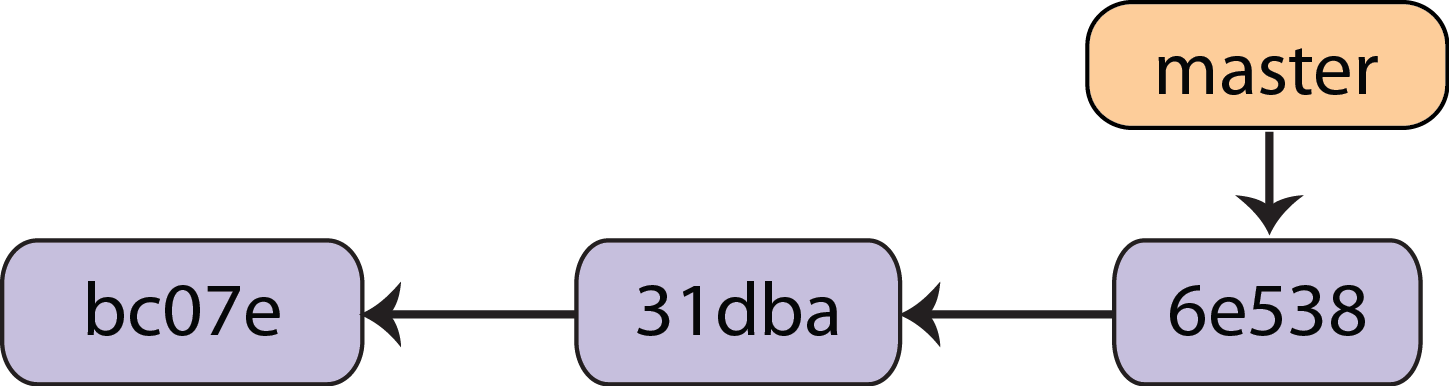
\includegraphics{../imgs/branch1.png}}

\vspace{20pt}
We have been using the \texttt{master} branch.
\end{center}

\end{frame}

\begin{frame}
\frametitle{Intro to Branching}
We can create a new branch and it will add a new pointer to the current commit:
\begin{center}
\scalebox{0.7}{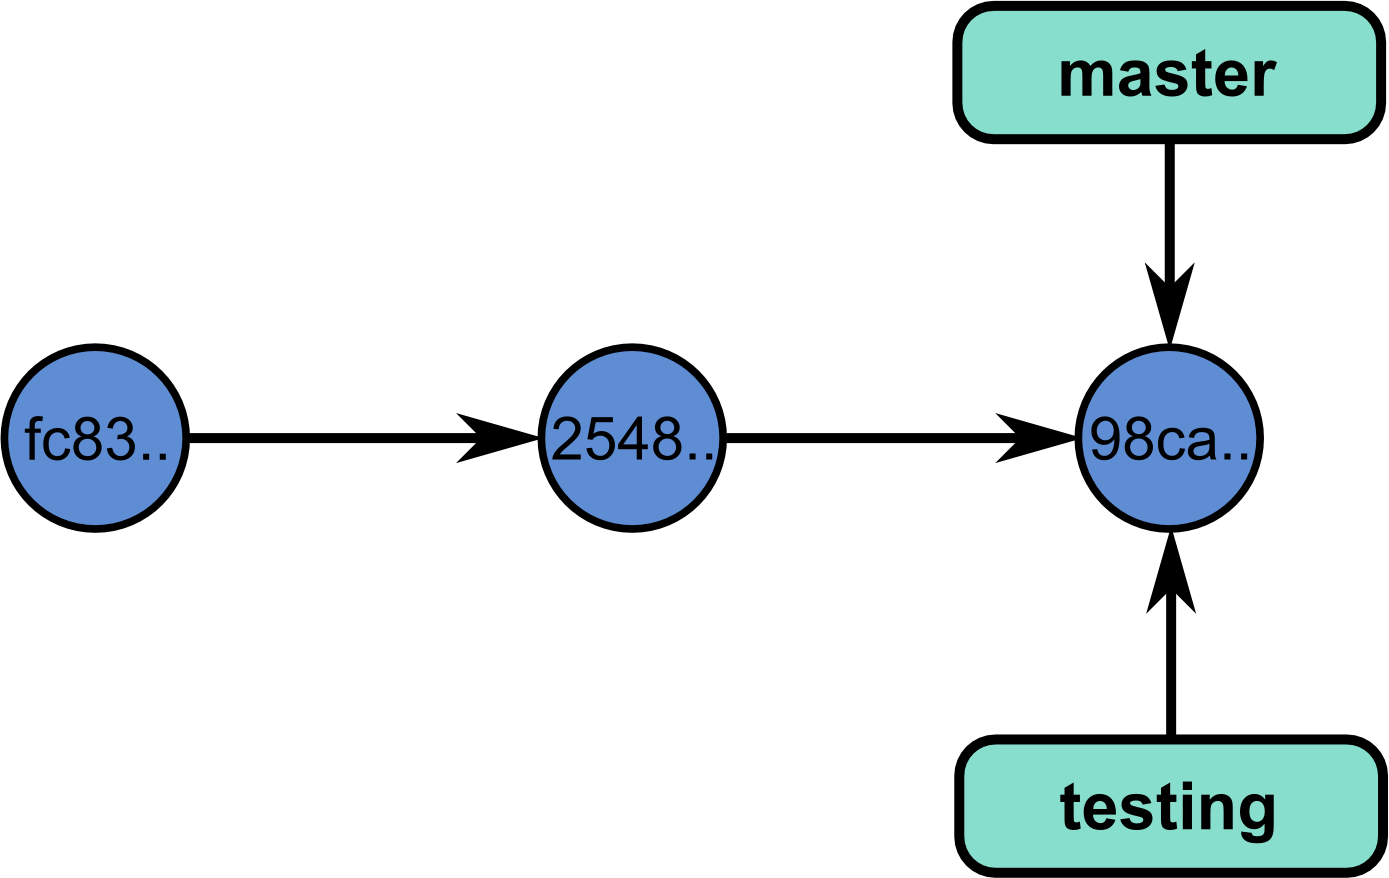
\includegraphics{../imgs/branch2.png}}

\end{center}
\end{frame}

\begin{frame}
\frametitle{Intro to Branching}
How does \texttt{Git} know which branch you are currently on? 
\begin{center}
\scalebox{0.6}{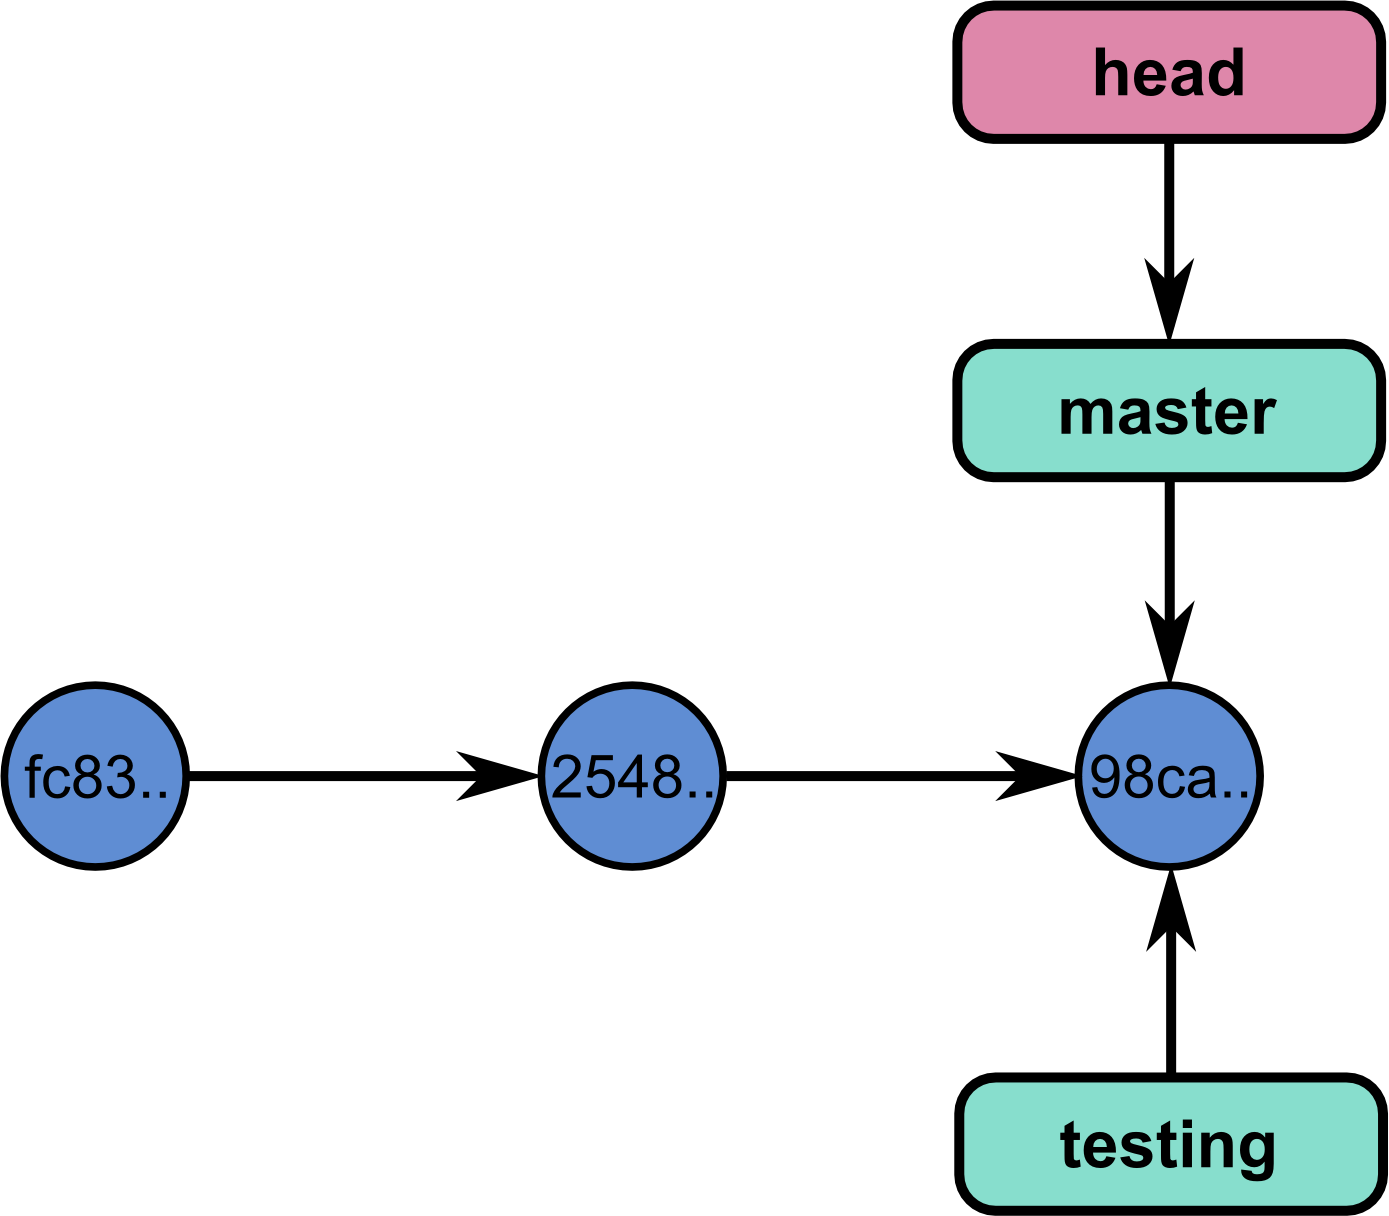
\includegraphics{../imgs/branch3.png}}

\end{center}
\end{frame}

\begin{frame}
\frametitle{Intro to Branching}
If you add commits on both branches, the directories can diverge:
\begin{center}
\scalebox{0.5}{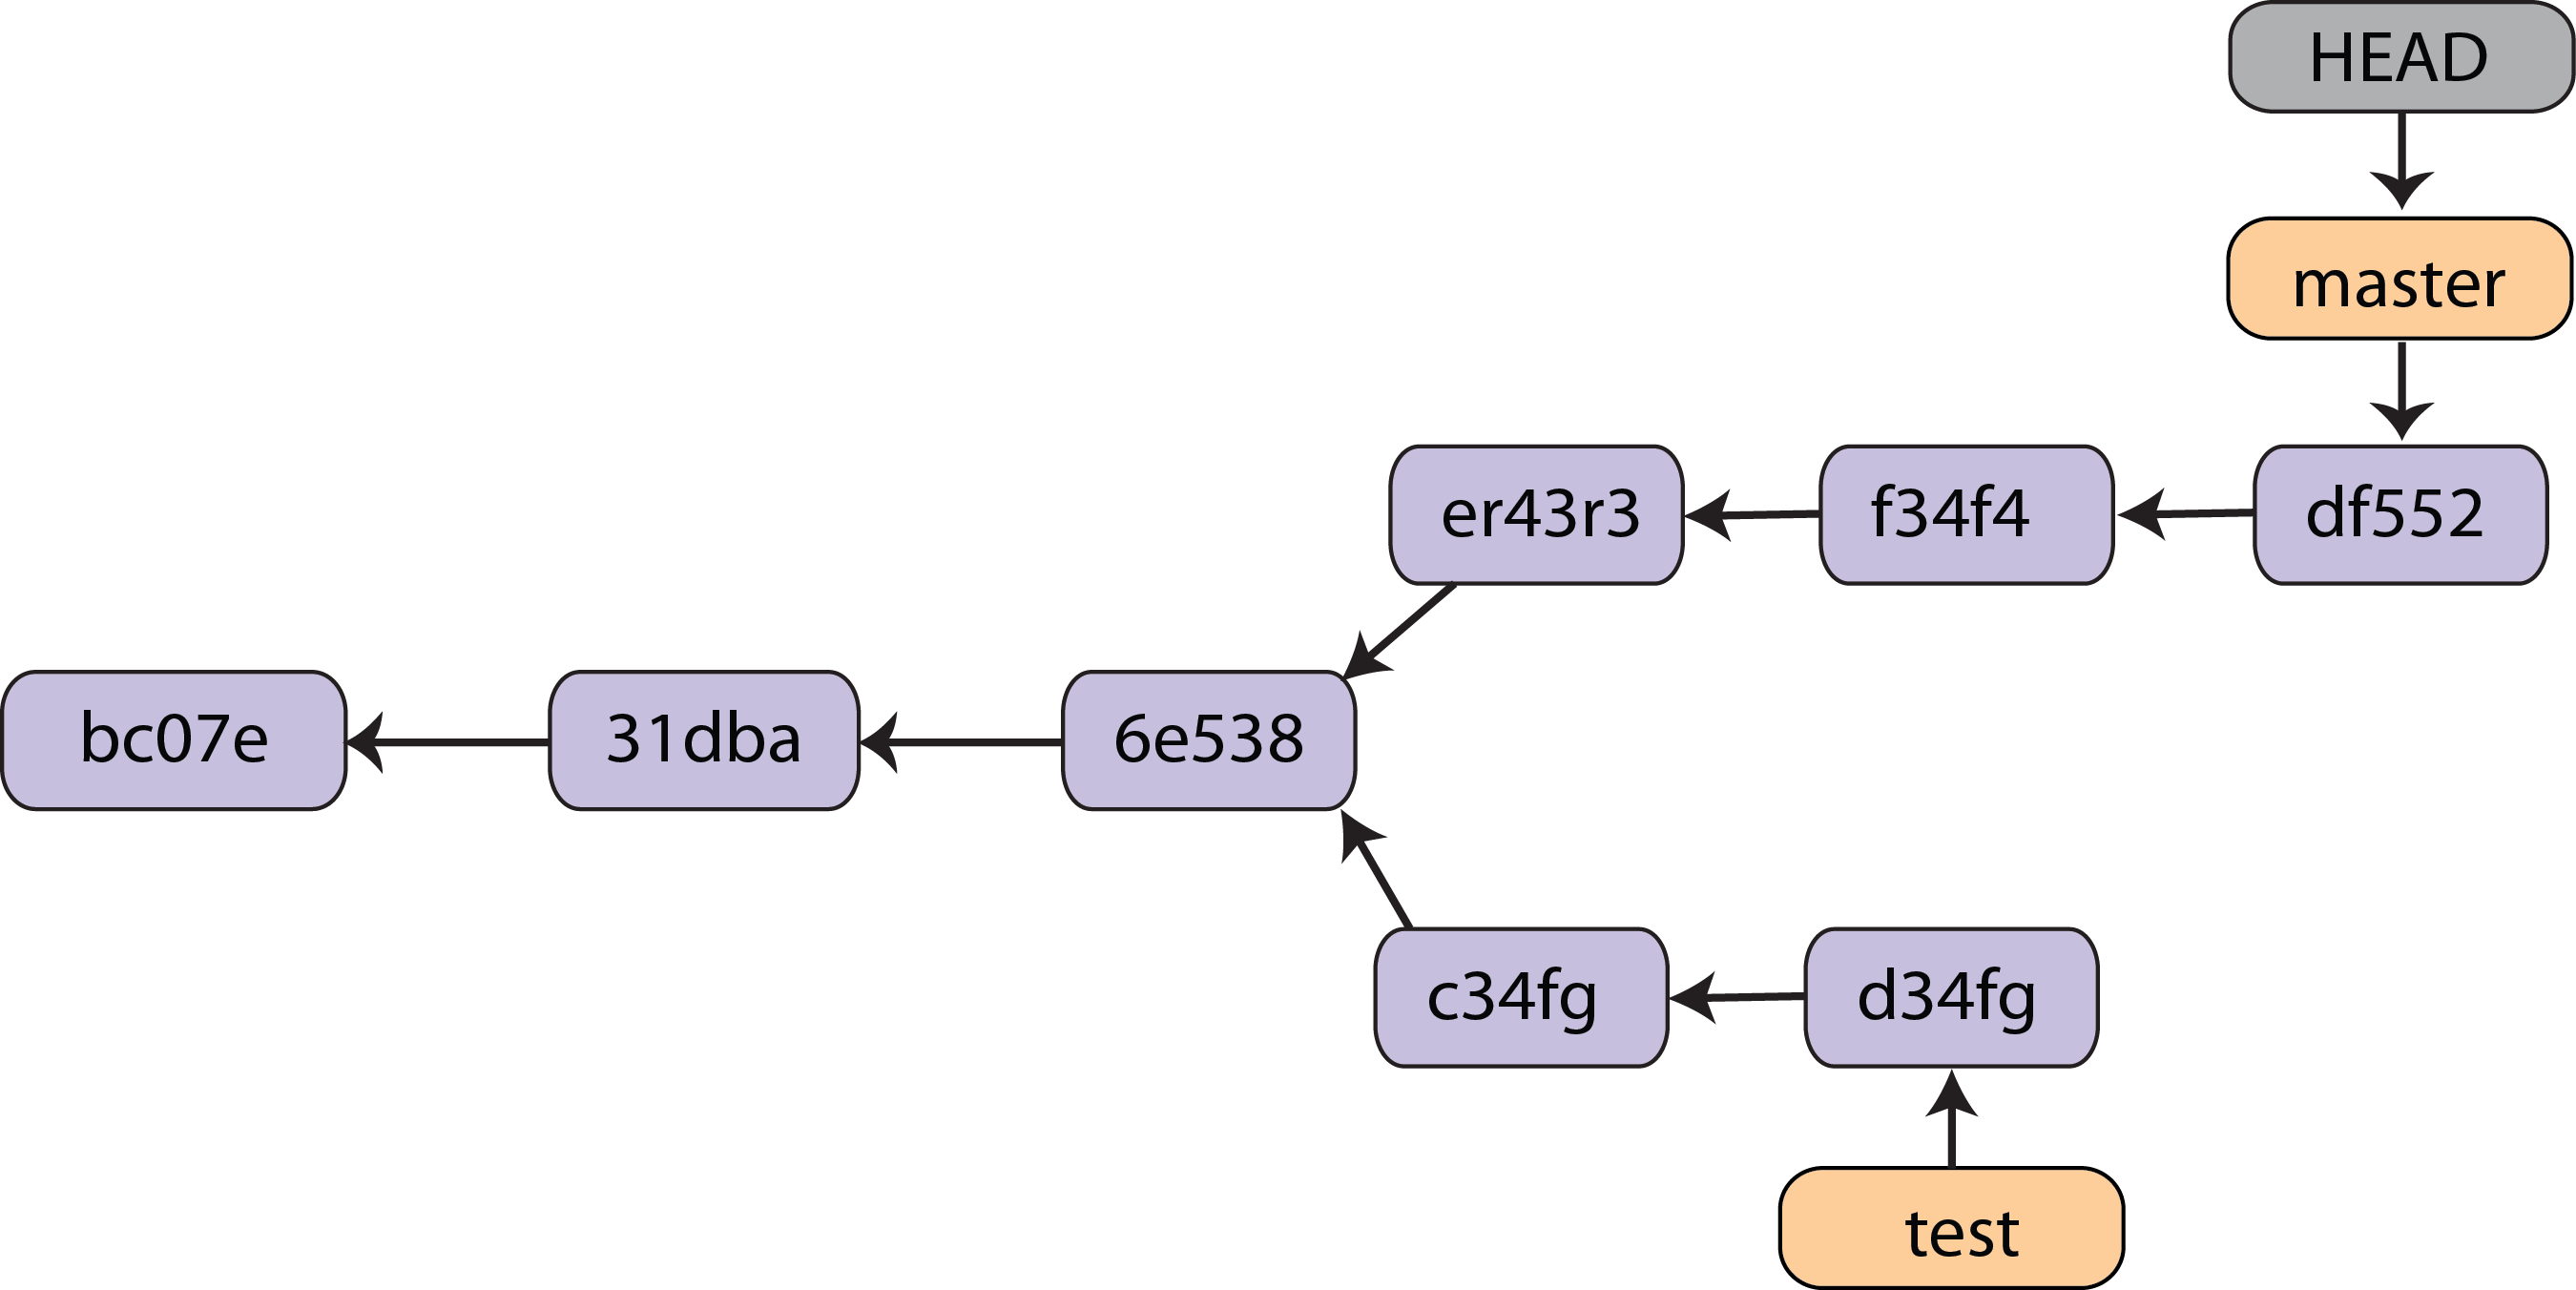
\includegraphics{../imgs/branch4.png}}

\end{center}
\end{frame}

\begin{frame}
\frametitle{Intro to Branching}
Eventually, you might want to merge your changes on your branch back into the master development branch:
\begin{center}
\scalebox{0.5}{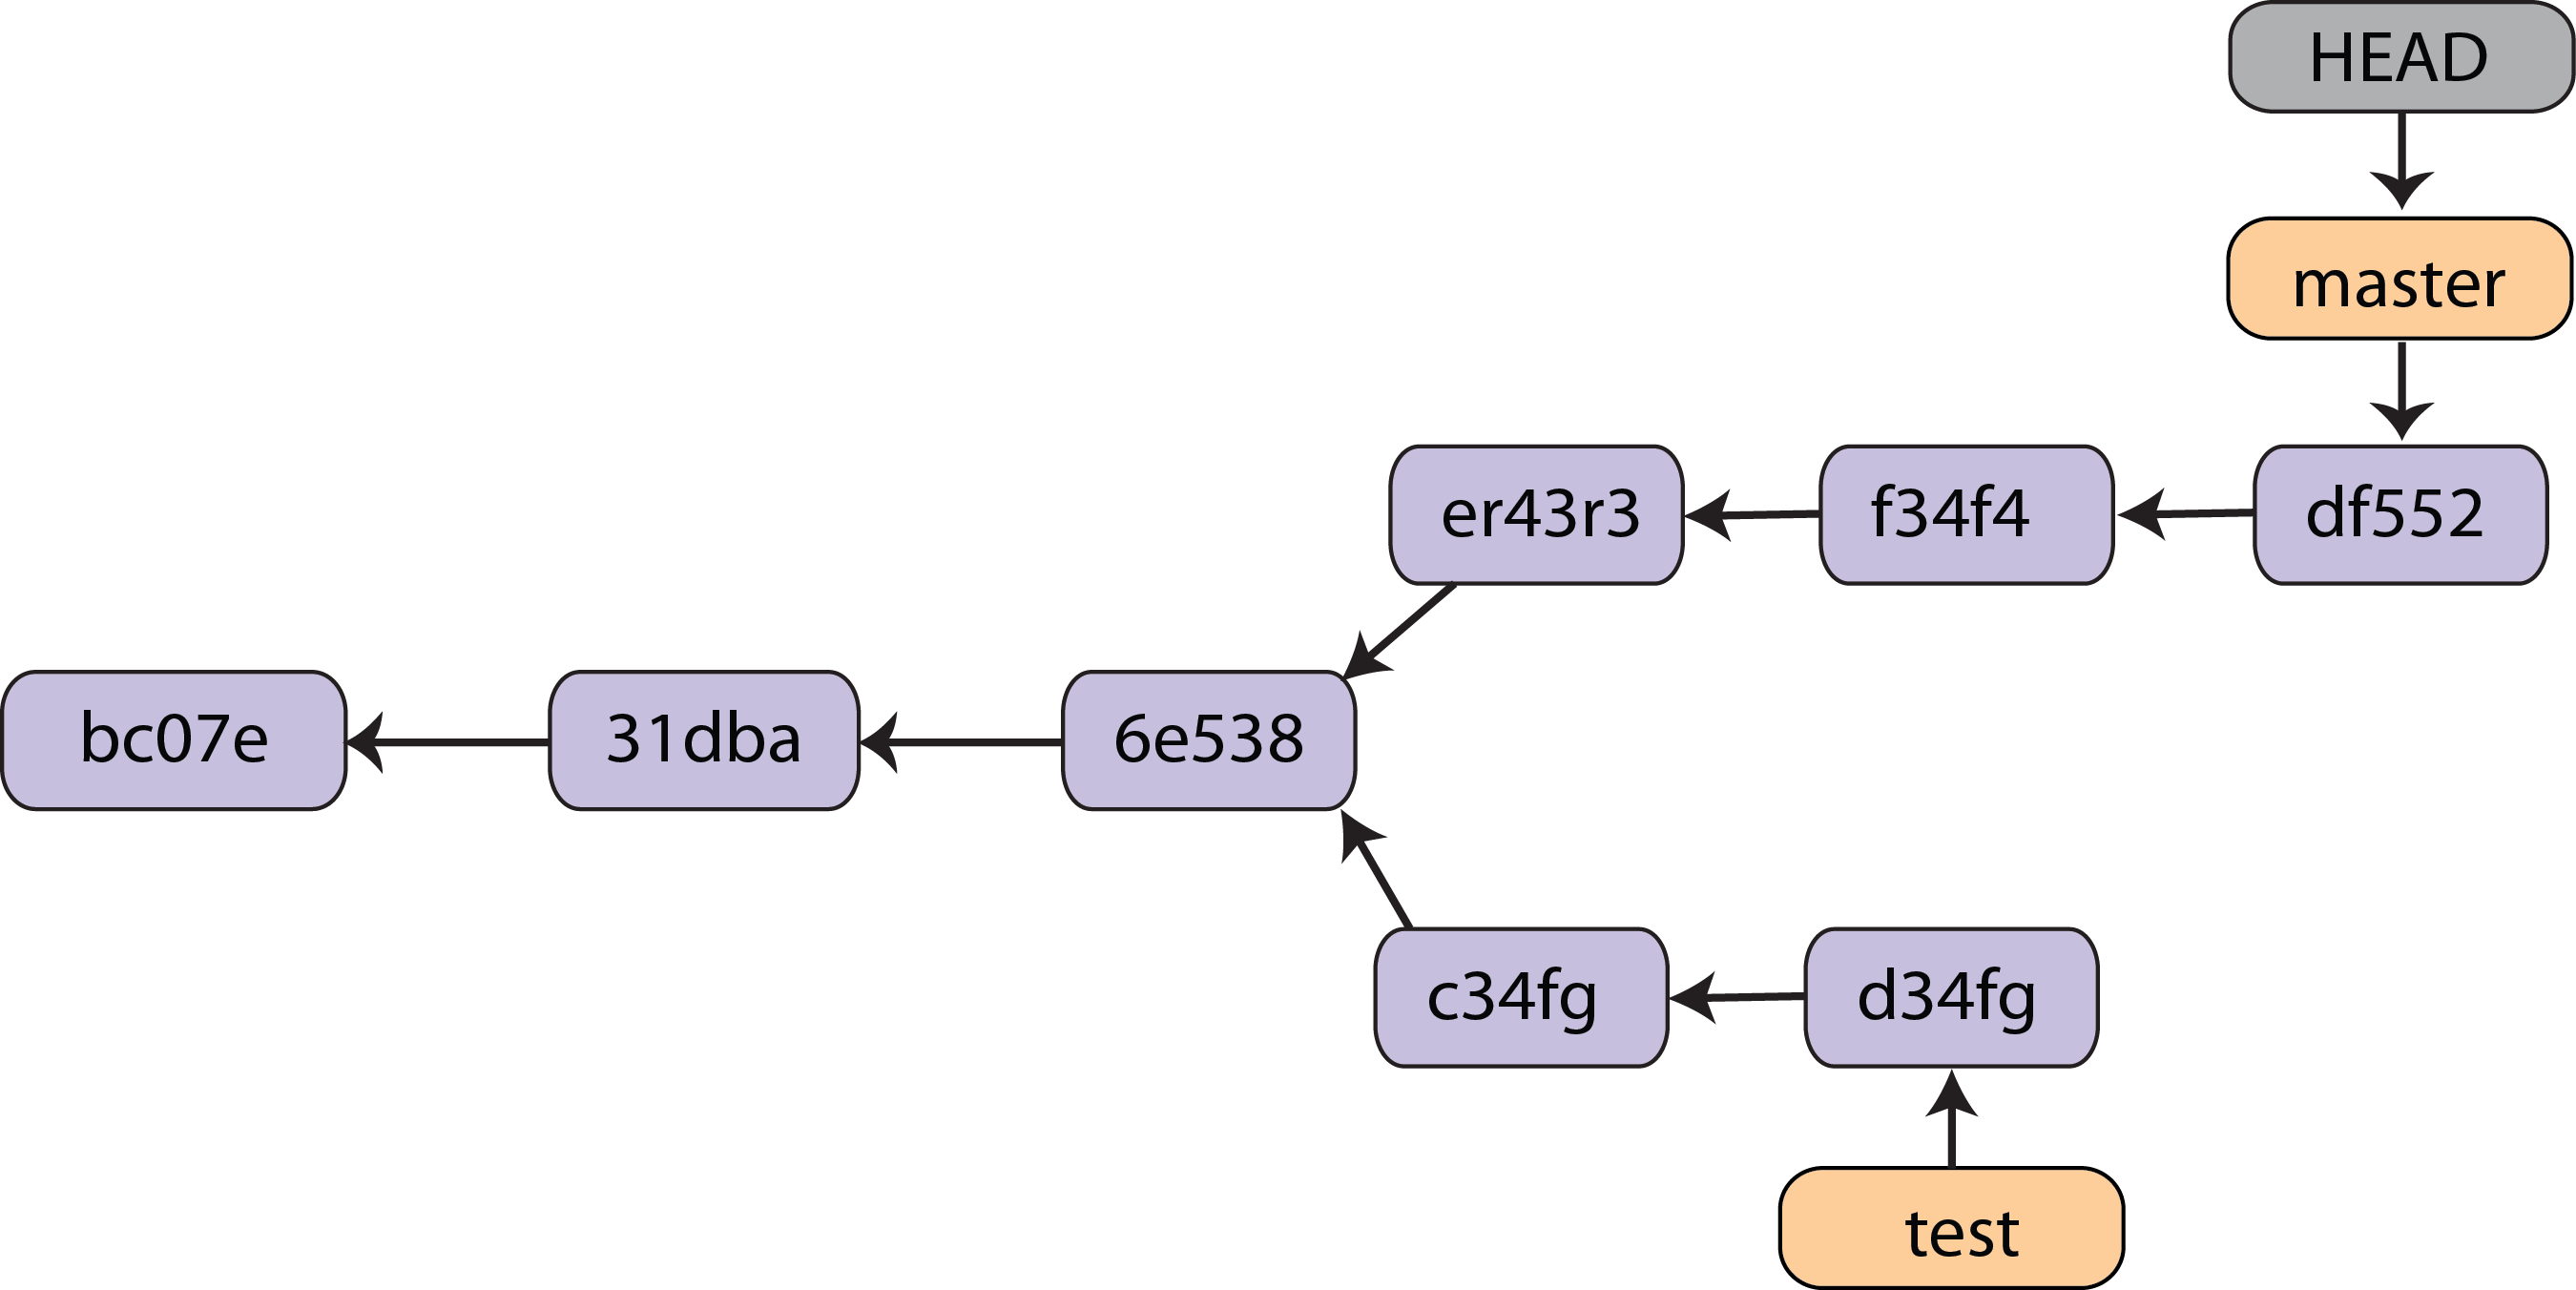
\includegraphics{../imgs/branch4.png}}

\end{center}
\end{frame}


\begin{frame}
\frametitle{Why branch?}
\begin{center}
Isolation of changes. \pause
\vspace{15pt}

Try new things without disrupting main code. 
\end{center} \pause

Usually, there are a few main types of branches:
\begin{enumerate}
\item Feature Branch
\begin{itemize}
\item If a particular feature is disruptive enough that you don't want the entire development team to be affected in its early stages, you can create a branch on which to do this work.
\end{itemize}
\item Fixes Branch
\begin{itemize}
\item While development continues on the main trunk, a fixes branch can be created to hold the fixes to the latest released version of the software.
\end{itemize}
\end{enumerate} 
\end{frame}

\begin{frame}
\frametitle{Now, how do we actually do this?}
\end{frame}

\begin{frame}
\frametitle{Resolving Conflicts}
\end{frame}

\begin{frame}
\frametitle{Your Turn}
\begin{center}
\textbf{\textcolor{red}{Exercise 5 (30 mins)}}
\end{center}
\end{frame}


\end{document}


